\documentclass[12pt,a4paper]{article}

\usepackage[utf8]{inputenc}
\usepackage[T1]{fontenc}
\renewcommand{\contentsname}{Contenido}
\setlength{\parindent}{0pt}
\emergencystretch=2em
\usepackage{amsmath,amssymb}
\usepackage[margin=2.3cm]{geometry}
\usepackage{xcolor}
\usepackage[most]{tcolorbox}
\usepackage{tabularx, array}
\usepackage{enumitem}
\usepackage{booktabs}
\usepackage{longtable}
\usepackage{fancyhdr}
\usepackage[hidelinks]{hyperref}
\usepackage{titlesec}
\usepackage{float}

\setlength{\parskip}{4pt}
\setlist{itemsep=1pt,topsep=3pt}
\setcounter{secnumdepth}{3}
\setcounter{tocdepth}{2}

\definecolor{azulprin}{RGB}{0,45,114}
\definecolor{rojoprin}{RGB}{190,0,20}

\titleformat{\section}{\Large\bfseries\color{azulprin}}{\thesection.}{0.6em}{}[\color{azulprin}\titlerule]
\titleformat{\subsection}{\large\bfseries\color{azulprin}}{\thesubsection}{0.6em}{}
\titleformat{\subsubsection}{\normalsize\bfseries\color{rojoprin}}{\thesubsubsection}{0.6em}{}

\pagestyle{fancy}
\fancyhf{}
\fancyhead[L]{\small Procesos de Manufactura}
\fancyhead[R]{\small Resumen de estudio -- Semanas 1 a 4}
\fancyfoot[C]{\thepage}
\renewcommand{\headrulewidth}{0.4pt}

% ---------- cajas ----------
\newtcolorbox{defi}[1][]{enhanced,breakable,colback=blue!4,colframe=azulprin,
  fonttitle=\bfseries\small,title={#1},boxrule=0.6pt,arc=2pt,left=6pt,right=6pt,top=3pt,bottom=3pt}
\newtcolorbox{formu}[1][]{enhanced,breakable,colback=yellow!12,colframe=orange!80!black,
  fonttitle=\bfseries\small,title={#1},boxrule=0.6pt,arc=2pt,left=6pt,right=6pt,top=3pt,bottom=3pt}
\newtcolorbox{aviso}[1][]{enhanced,breakable,colback=red!5,colframe=rojoprin,
  fonttitle=\bfseries\small,title={#1},boxrule=0.6pt,arc=2pt,left=6pt,right=6pt,top=3pt,bottom=3pt}
\newtcolorbox{compl}[1][]{enhanced,breakable,colback=green!5,colframe=green!40!black,
  fonttitle=\bfseries\small,title={#1},boxrule=0.6pt,arc=2pt,left=6pt,right=6pt,top=3pt,bottom=3pt}

\newcommand{\ud}[1]{\,\mathrm{#1}}

\title{\textbf{\color{azulprin}Procesos de Manufactura}\\[10pt]
\large Resumen de estudio -- Semanas 1 a 4}
\author{Luis Alejandro Rey de Castro}
\date{}

\begin{document}
\maketitle
\thispagestyle{fancy}

% =====================================================================
\section{Semana 1: Propiedades de los materiales, estructura cristalina y
  defectos}
% =====================================================================

\subsection{Tipos de materiales y su evolución}

Los materiales para ingeniería se clasifican en cuatro grandes familias:
\textbf{metales, cerámicos, polímeros y compuestos}.

La \textbf{transformación de los materiales} sigue una cadena típica (ejemplo
del avión): extracción del mineral $\rightarrow$ alto horno (obtención del
metal) $\rightarrow$ colada/fundición $\rightarrow$ tratamiento
térmico/conformado (desarrollo de microestructura de granos) $\rightarrow$
ensamblaje $\rightarrow$ producto final.

\textbf{Evolución histórica}: la importancia relativa de cada familia ha
cambiado con el tiempo.
\begin{itemize}
	\item \textbf{Metales:} oro, cobre, bronce, hierro $\rightarrow$ fundición,
	      aceros $\rightarrow$ aleación de aceros $\rightarrow$ aleaciones
	      ligeras,
	      superaleaciones, titanio, circonio $\rightarrow$ metales vítreos,
	      aleaciones
	      Al--Li, aceros de fase dual, aceros microaleados, nuevas
	      superaleaciones. Desde
	      los 80--90 el desarrollo es lento: principalmente control de calidad y
	      procesado.
	\item \textbf{Cerámicos y vidrios:} piedra, pedernal, loza, vidrio
	      $\rightarrow$ cemento, refractarios $\rightarrow$ cemento Portland,
	      sílice
	      fundida $\rightarrow$ cerámicas técnicas tenaces (Al$_2$O$_3$,
	      Si$_3$N$_4$,
	      PSZ), pirocerámicas.
	\item \textbf{Polímeros / elastómeros:} madera, pieles, fibras, colas
	      $\rightarrow$ caucho $\rightarrow$ baquelita $\rightarrow$ nylon, PE
	      (polietileno), PMMA, PC (policarbonato), PS, PP, acrílicos, epoxis,
	      poliésteres $\rightarrow$ polímeros de alto módulo y para altas
	      temperaturas.
	\item \textbf{Materiales compuestos:} adobe $\rightarrow$ GFRP, CFRP,
	      Kevlar-FRP $\rightarrow$ compuestos cerámicos y de matriz metálica
	      $\rightarrow$ fibra de carbono y hormigón armado.
\end{itemize}

\subsection{Proceso de selección de un material}

\begin{defi}[Idea central]
	\emph{``No hay material malo, sino mal diseñado, mal seleccionado y/o mal
		utilizado.''}
\end{defi}

El diagrama de selección relaciona:
\begin{enumerate}
	\item \textbf{Uso o aplicación} $\rightarrow$ define las \textbf{condiciones
		      de trabajo}.
	\item Las condiciones de trabajo generan \textbf{deterioro y desgaste}, lo que
	      retroalimenta las condiciones de trabajo y las propiedades requeridas.
	\item \textbf{Propiedades requeridas por el producto} y \textbf{presupuesto}
	      $\rightarrow$ \textbf{elección del material}.
\end{enumerate}

\textbf{El progreso tecnológico plantea nuevas necesidades} y exige materiales:
más fuertes, más livianos, más tenaces, más durables; que no contaminen el medio
ambiente; que sean reciclables; de fácil procesamiento; y económicamente de bajo
costo.

\textbf{Conocimiento científico que involucra la selección} (de lo atómico a lo
macroscópico): (1) la estructura de los materiales, (2) los constituyentes de un
material, (3) los procesos de transformación, (4) las propiedades mecánicas,
físicas y químicas.

\subsection{Estructura cristalina}

\begin{defi}[Materiales cristalinos vs.\ amorfos]
	Los \textbf{metales, algunos cerámicos y polímeros} al \textbf{solidificarse
		se
		organizan en una red cristalina}. Los \textbf{materiales cristalinos} tienen
	una
	\textbf{estructura organizada} (orden de largo alcance), a diferencia de los
	\textbf{materiales amorfos}, que \textbf{no tienen orden}.
\end{defi}

Imágenes de microscopía (MEV) usadas como ejemplo: frontera entre dos cristales
de TiO$_2$ (organización geométrica de sus átomos); carbono amorfo
(desorganización en la posición de sus átomos); titanio y Al$_2$O$_3$ (redes
ordenadas).

\subsubsection{Tipos de estructuras cristalinas: 14 redes de Bravais}
Existen \textbf{14 redes de Bravais}. Las tres más conocidas (las de los metales
comunes) son:

\begin{center}
	\small
	\begin{tabularx}{\linewidth}{llX}
		\toprule
		\textbf{Estructura}    &
		\textbf{Ejemplos}      &
		\textbf{Propiedades mecánicas}
		\\
		\midrule
		BCC                    &
		Fe-$\alpha$, Cr, W, Mo &
		Alta resistencia y dureza; menor ductilidad que FCC
		\\
		FCC                    &
		Al, Cu, Ni, Ag, Au     &
		Muy dúctil y maleable; fácil deformación plástica
		\\
		HCP                    &
		Mg, Zn, Ti, Co         &
		Menor ductilidad; deformación plástica más limitada
		\\
		\bottomrule
	\end{tabularx}
\end{center}

\subsubsection{Estructura cristalina de los metales}

\begin{defi}[I. Cúbico centrado en el cuerpo (BCC)]
	Los átomos ocupan \textbf{los vértices} y \textbf{un átomo en el centro del
		cubo}, siendo tangentes a lo largo de las \textbf{diagonales del cubo}.
	$$2 \text{ átomos por celda} = 8 \times \dfrac{1}{8} + 1 \times 1$$
\end{defi}

\begin{defi}[II. Cúbico centrado en las caras (FCC)]
	Los átomos ocupan \textbf{los vértices y el centro de las caras} de un cubo,
	siendo tangentes a lo largo de las \textbf{diagonales de las caras}.
	$$4 \text{ átomos por celda} = 8 \times \dfrac{1}{8} + 6 \times \dfrac{1}{2}$$
\end{defi}

\begin{defi}[III. Hexagonal compacta (HCP)]
	Los átomos ocupan \textbf{los vértices de un prisma hexagonal regular},
	\textbf{los centros de las bases} y \textbf{los centros de los triángulos} en
	que puede descomponerse la sección media del prisma. (Parámetros de red: $a$ y
	$c$.)
	$$6 \text{ átomos por celda} = 12 \times \dfrac{1}{6} + 2 \times \dfrac{1}{2}
		+
		3 \times 1$$
\end{defi}

\begin{figure}[h!]
	\centering
	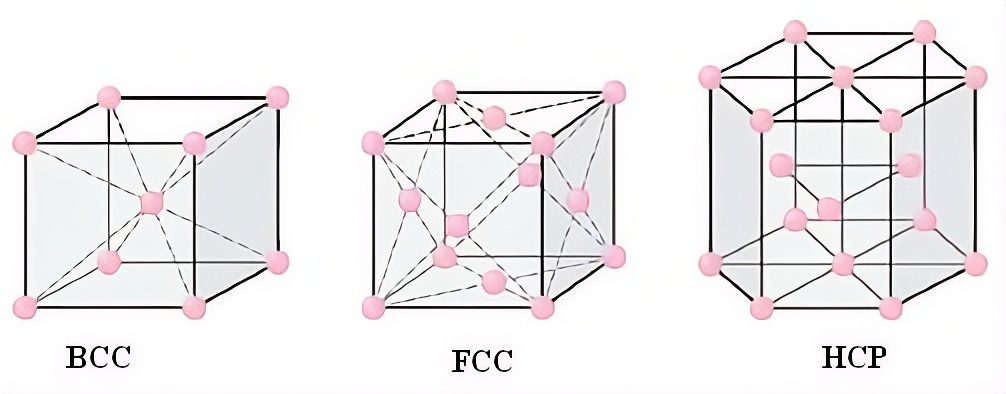
\includegraphics[width=0.8\linewidth]{img/lattice.jpeg}
\end{figure}

\subsection{Defectos e imperfecciones en estructuras cristalinas}

\begin{defi}[¿Qué es un defecto?]
	Las imperfecciones (también llamadas \textbf{defectos}) son \textbf{cualquier
		fallo o interrupción del orden cristalino, ya sea de corto o largo alcance}.
	\textbf{Modifican las propiedades de los materiales.}
\end{defi}

Realmente \textbf{no existen cristales perfectos}: contienen varios tipos de
imperfecciones y defectos que afectan sus \textbf{propiedades físicas y
	mecánicas} y que influyen en propiedades de aplicación en ingeniería como: la
capacidad de formar aleaciones en frío, la conductividad eléctrica y la
corrosión.

\subsubsection{Clasificación de defectos según su dimensión}

\begin{center}
	\begin{tabularx}{\linewidth}{lX}
		\toprule
		\textbf{Tipo}              & \textbf{Defectos incluidos}
		\\
		\midrule
		\textbf{Puntuales} (0D)    & Vacantes, intersticiales, sustitucional,
		Schottky, Frenkel
		\\
		\textbf{Lineales} (1D)     & Dislocación de arista, de hélice y mixtas    \\
		\textbf{Planares} (2D)     & \emph{Estructurales:} superficies, bordes de
		grano, plano de macla, falta de apilamiento. \emph{De composición:} planos de
		cizalladura cristalográfica, planos de macla química                      \\
		\textbf{Volumétricos} (3D) & Poros, grietas, inclusiones (y rechupes en
		piezas fundidas)
		\\
		\bottomrule
	\end{tabularx}
\end{center}

\subsubsection{Defectos puntuales}

\begin{description}[leftmargin=0pt,style=nextline]
	\item[1. Vacante] \textbf{Ausencia de un átomo} en la estructura cristalina
	      (un sitio de la red queda vacío).
	\item[2. Intersticial] Se forma cuando se \textbf{inserta un átomo o ion
		      adicional} en la estructura cristalina, normalmente en una
	      \textbf{posición
		      desocupada} (entre los átomos de la red). Si el átomo es del mismo
	      material se
	      llama \emph{autointersticial} (\emph{self-interstitial}).
	\item[3. Sustitucional (o impurezas en sólidos)] Un átomo/ion es
	      \textbf{sustituido por un átomo o ion de tipo distinto}. El átomo puede
	      ser
	      \textbf{más pequeño o más grande} que el original, y en ambos casos
	      distorsiona
	      la red (átomo sustitucional pequeño $\Rightarrow$ la red se contrae
	      alrededor;
	      grande $\Rightarrow$ se expande).
	\item[4. Defecto Frenkel] Imperfección \textbf{combinada
		      vacancia--intersticial}: un ion salta de un punto normal de la red a
	      un sitio
	      intersticial, dejando una vacancia. Es decir, \textbf{vacante + catión
		      intersticial}. Ocurre con \textbf{iones pequeños} (H y Li). Ejemplo:
	      \textbf{haluros de plata}.
	\item[5. Defecto Schottky] Es un \textbf{par de vacancias} en un material con
	      \textbf{enlaces iónicos}. Para mantener la \textbf{neutralidad
		      eléctrica} deben
	      perderse de la red \textbf{tanto un catión como un anión} (vacantes
	      catiónicas y
	      aniónicas). Ejemplo: \textbf{haluros alcalinos}.
\end{description}

\begin{aviso}[Para no confundir Frenkel con Schottky]
	\textbf{Frenkel} = el ion \emph{se mueve} dentro del cristal (vacante +
	intersticial, el ion sigue en el cristal). \textbf{Schottky} = el par
	catión--anión \emph{sale} de la red (dos vacantes, una de cada signo).
\end{aviso}

\subsubsection{Defectos lineales (dislocaciones)}

\textbf{Característica:} se pueden \textbf{desplazar} en el interior del cristal
con \textbf{esfuerzos mecánicos relativamente bajos} y producir el
desplazamiento completo de planos cristalinos.

\textbf{Qué explican:} la \textbf{deformación plástica en los metales}
(maleabilidad, ductilidad, etc.).

\textbf{Cómo se forman:}
\begin{itemize}
	\item Durante la solidificación y el enfriamiento.
	\item Por deformación plástica del sólido.
	\item Por condensación de vacantes.
	\item Por desajustes atómicos en soluciones sólidas.
\end{itemize}

\begin{description}[leftmargin=0pt,style=nextline]
	\item[1. Dislocación de arista (borde, cuña o de Taylor)] Modificación
	      geométrica debida a un \textbf{plano atómico adicional} (un semiplano
	      extra de átomos insertado en la red). Se caracteriza por la línea de
	      dislocación y el \textbf{vector de Burgers} ($\mathbf b$, vector de
	      deslizamiento,
	      $\mathbf b \perp$ línea de dislocación.)
	\item[2. Dislocación de hélice (tornillo o de Burgers)] Modificación debida a
	      \textbf{esfuerzos de cizalladura}; produce una \textbf{distorsión en
		      forma de espiral} ($\mathbf b \parallel$ línea de dislocación).
	\item[3. Dislocación mixta] \textbf{Combinación de las anteriores} (es lo que
	      se encuentra en los materiales reales). \textbf{Finalizan en la
		      superficie, jamás dentro del cristal.} El vector $\mathbf b$
	      \textbf{no es paralelo ni perpendicular} a la línea de dislocación
	      (ángulo intermedio).
\end{description}

\begin{figure}[h!]
	\centering
	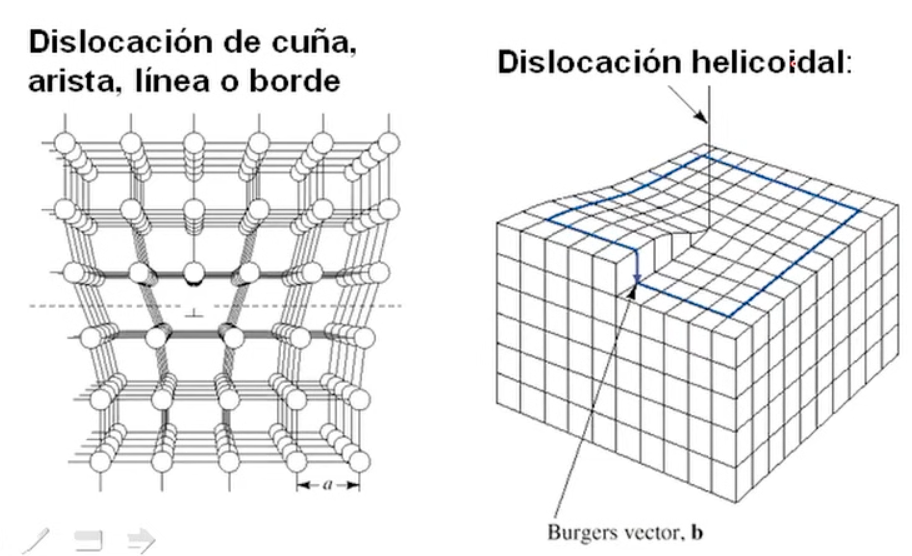
\includegraphics[width=0.7\linewidth]{img/defectos-lineales.png}
\end{figure}

\subsubsection{Defectos planares (interfaciales)}

\begin{description}[leftmargin=0pt,style=nextline]
	\item[1. Borde o límite de grano] Frontera entre dos cristales (granos) de
	      distinta orientación dentro de un mismo material policristalino; se
	      observa en
	      micrografías como líneas que delimitan polígonos irregulares.
	\item[2. Planos de macla] Plano que separa dos partes de un mismo grano con
	      una pequeña diferencia de orientación (\textbf{macla = imagen especular
		      de dos
		      redes respecto del plano de la macla}). Dentro de un grano, la
	      aplicación de un
	      esfuerzo cortante puede desplazar levemente los átomos a lo largo de la
	      macla.
	      \textbf{Formación:} durante procesos de deformación o en tratamientos
	      térmicos.
	      Producen un aumento de la resistencia mecánica $\Rightarrow$ materiales
	      \emph{menos} deformables plásticamente (menos dúctiles).
	\item[3. Límites de fase] Interfaz entre dos fases distintas presentes en la
	      microestructura (por ejemplo, zonas de distinto tono en una
	      micrografía).
\end{description}

\subsubsection{Defectos volumétricos}
Poros, grietas e inclusiones. En piezas fundidas aparecen además
\textbf{rechupes}. Las grietas pueden ser \textbf{macrogrietas} o
\textbf{microgrietas}. Las inclusiones son partículas de otro material
incorporadas durante el procesamiento.

% =====================================================================
\section{Semana 2: Dimensiones, tolerancias y superficies}
% =====================================================================

\subsection{Introducción}
Por las inexactitudes de los métodos de producción es \textbf{imposible fabricar
	piezas con exactamente las dimensiones elegidas en el diseño}, y que todas las
piezas de una producción en serie queden con dimensiones idénticas. Por tanto,
se debe \textbf{aceptar cierta variación en las medidas}. Cuando se requiere
exactitud (por ejemplo, para montajes), es necesario un \textbf{control de las
	dimensiones}.

El diseñador especifica tres atributos de un producto:
\begin{center}
	\begin{tabular}{@{}p{5cm}p{5cm}p{5cm}@{}}
		\toprule
		\textbf{Dimensiones} & \textbf{Tolerancias}                    &
		\textbf{Superficies}
		\\
		\midrule
		Tamaños lineales o angulares de un componente, especificados en el plano de
		la
		pieza.               & Una variación limitada de la dimensión. & Límite
		exterior de un objeto
		con su ambiente, que puede ser otro objeto, un fluido, el espacio o una
		combinación de éstos.                                                   \\
		\bottomrule
	\end{tabular}
\end{center}

\begin{defi}[Definiciones ANSI]
	\textbf{Dimensión:} valor numérico expresado en las unidades apropiadas de
	medida, que se indica en un plano y otros documentos junto con líneas,
	símbolos
	y notas para definir el tamaño o característica geométrica (o ambas) de una
	pieza.\\[3pt]
	\textbf{Tolerancia:} la cantidad total que está permitido que una dimensión
	específica varíe. \textbf{Es la diferencia entre los límites máximo y mínimo.}
\end{defi}

\subsection{Formas de especificar una tolerancia}
\begin{itemize}
	\item \textbf{Tolerancia bilateral:} la variación es en las direcciones
	      \textbf{positiva y negativa} a partir de la dimensión nominal. Ejemplo:
	      $2.500\,^{+0.005}_{-0.005}$ (o $2.500 \pm 0.005$).
	\item \textbf{Tolerancia unilateral:} la variación a partir de la dimensión
	      especificada se permite \textbf{sólo en una dirección} (positiva o
	      negativa).
	      Ejemplo: $2.500\,^{+0.010}_{-0.000}$.
	\item \textbf{Tolerancia límite:} consiste en las \textbf{dimensiones máxima y
		      mínima permitidas}. Ejemplo: $2.505 / 2.495$.
\end{itemize}

Además, las tolerancias se clasifican en \textbf{dimensionales} (asociadas al
tamaño) y \textbf{geométricas} (forma, orientación, posición).

\subsection{Tolerancia dimensional}
Está asociada al concepto de \textbf{tamaño} (diámetro o distancia entre dos
planos paralelos) y establece los \textbf{límites permisibles para el tamaño de
	una característica}. Se usa en sistemas normalizados de tolerancia y ajustes:
eje/agujero, conos, engranajes, pernos y tornillos.

\begin{itemize}
	\item \textbf{Dimensión:} cifra que expresa el valor numérico de una longitud
	      o un ángulo.
	\item \textbf{Dimensiones límites:} valores extremos que puede tomar la
	      dimensión efectiva.
	\item \textbf{Diferencia o desviación:} diferencia entre una dimensión y la
	      dimensión nominal. \textbf{Diferencia efectiva} = medida efectiva $-$
	      nominal.
	\item \textbf{Línea de referencia o línea cero:} recta que sirve de referencia
	      para las desviaciones y que corresponde a la dimensión nominal.
	\item \textbf{Diferencia fundamental:} una cualquiera de las desviaciones
	      límites (superior o inferior), elegida convenientemente para definir la
	      \textbf{posición de la zona de tolerancia} respecto a la línea cero.
	\item \textbf{Zona de tolerancia:} zona cuya amplitud es el valor de la
	      tolerancia.
	\item \textbf{Tolerancia fundamental:} la que se determina para cada grupo de
	      dimensiones y para cada calidad de trabajo (grado IT).
\end{itemize}

\begin{defi}[Eje y agujero]
	Pareja de elementos, uno \textbf{macho (eje)} y otro \textbf{hembra
		(agujero)}, que encajan entre sí, independientemente de la forma de la
	sección
	que tengan.
\end{defi}

\subsubsection{Terminología y notación}
Convención: \textbf{minúsculas para ejes}, \textbf{MAYÚSCULAS para agujeros}.

\begin{center}
	\small
	\begin{tabularx}{\linewidth}{lllX}
		\toprule
		\textbf{Concepto}   & \textbf{Eje} & \textbf{Agujero} &
		\textbf{Significado}
		\\
		\midrule
		Dimensión nominal   & $d_N$        & $D_N$            & Valor
		teórico respecto al que se consideran las medidas límites
		\\
		Dimensión efectiva  & $d_e$        & $D_e$            & Valor
		real, medido sobre la pieza ya construida
		\\
		Dimensión máxima    & $d_M$        & $D_M$            & Valor
		extremo superior de la dimensión
		efectiva
		\\
		Dimensión mínima    & $d_m$        & $D_m$            & Valor
		extremo inferior de la dimensión
		efectiva
		\\
		Diferencia superior & $d_s$        & $D_s$            & Dim.\
		máxima $-$ nominal
		\\
		Diferencia inferior & $d_i$        & $D_i$            & Dim.\
		mínima $-$ nominal                                            \\
		Tolerancia          & $t$          & $T$              &
		Variación máxima permitida de la medida
		\\
		\bottomrule
	\end{tabularx}
\end{center}

\begin{figure}[h!]
	\centering
	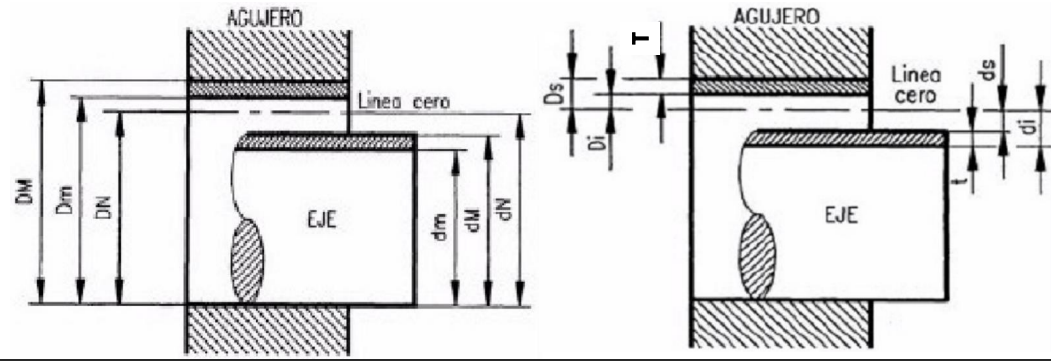
\includegraphics[width=\linewidth]{img/dimensiones.png}
\end{figure}

\begin{formu}[Relaciones fundamentales]
	\centering
	\begin{tabular}{@{}p{7cm}p{7cm}@{}}
		\textbf{Agujeros}           & \textbf{Ejes}               \\[2pt]
		$D_s = D_i + T$             & $d_s = d_i + t$             \\[2pt]
		$D_M = D_m + T$             & $d_M = d_m + t$             \\[2pt]
		$T = D_M - D_m = D_s - D_i$ & $t = d_M - d_m = d_s - d_i$ \\[2pt]
		$D_M = D_N + D_s$           & $d_M = d_N + d_s$           \\[2pt]
		$D_m = D_N + D_i$           & $d_m = d_N + d_i$           \\
	\end{tabular}
\end{formu}

\subsubsection{Ejemplo}

(Como el eje siempre es menor que el agujero, es un ajuste con juego; ver más
abajo: $J_M = 50.03 - 49.95 = 0.08$, $J_m = 50.01 - 49.98 = 0.03$, $T_J = 0.05 =
	T + t$.)

\begin{figure}[h!]
	\centering
	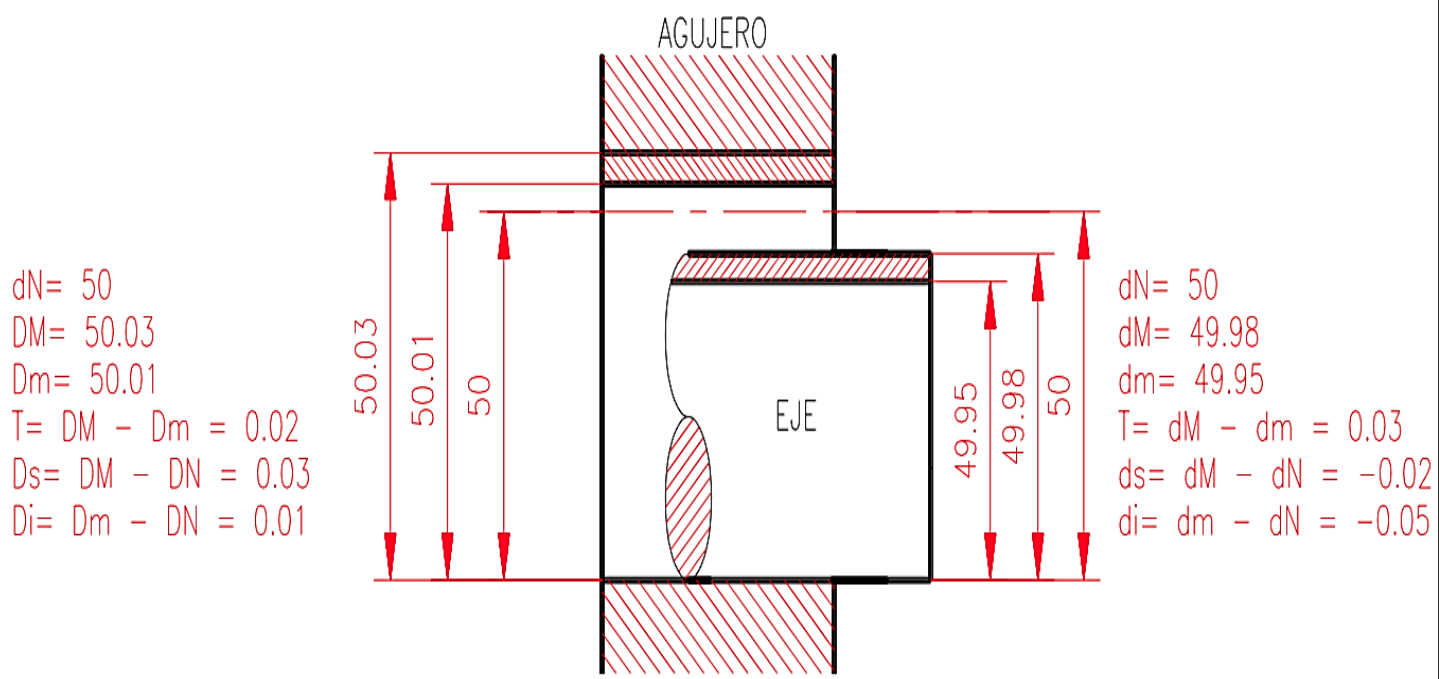
\includegraphics[width=\linewidth]{img/ejemplo-eje.png}
\end{figure}

\subsection{Representación de la tolerancia}
\textbf{Tolerancia lineal:} se puede representar de tres maneras:
\begin{enumerate}
	\item \textbf{Mediante símbolos ISO:} por ejemplo \textbf{30 H 6} = diámetro
	      nominal (30) + \textbf{posición de la tolerancia} (letra H -- desviación
	      inferior es 0 en el agujero) + \textbf{calidad de la tolerancia} (IT6 --
	      tolerancia de 0.013 mm / 13 $\mu$m, es decir, de 30.000 a 30.013 mm).
	\item \textbf{Mediante sus desviaciones admisibles:} por ejemplo
	      $32\,^{+0.1}_{-0.2}$, $32 \pm 0.1$, $32\,^{\,0}_{-0.2}$.
	\item \textbf{Mediante sus medidas límites:} por ejemplo $32.198 / 32.195$, o
	      ``30.5 mín.''
\end{enumerate}
\textbf{Tolerancia angular:} se expresa con desviaciones en
grados/minutos/segundos, por ejemplo $30^\circ\,^{+0^\circ 0' 15''}_{-0^\circ 0'
		30''}$, $60^\circ 10' \pm 0^\circ 0' 30''$, $15.5^\circ \pm 0.25^\circ$.

\subsection{Calidad de la tolerancia: grados IT}
Se han previsto \textbf{20 grados o índices de tolerancia (IT)}: IT01, IT0, IT1,
\ldots, IT18, que representan la \textbf{calidad} de la tolerancia,
\textbf{desde la más fina hasta la más basta}. Sus valores numéricos están
calculados para cada grupo de diámetros nominales y constituyen las
\textbf{tolerancias fundamentales} del sistema. Los grados \textbf{IT01 e IT0}
se consideran idóneos para \textbf{patrones de medida}.

Valores habituales de referencia: IT01--IT0 patrones; IT1--IT4 calibres y
piezas de gran precisión; IT5--IT12 piezas que ajustan; IT13--IT18 piezas que
no ajustan. \textbf{A menor número IT, menor tolerancia (más preciso y más
	caro de fabricar).}

\subsection{Posición de la zona de tolerancia (norma UNE-EN 20286-1 / ISO
	286-1)}
\begin{itemize}
	\item \textbf{En el agujero (letras MAYÚSCULAS):} de \textbf{A a H} la zona de
	      tolerancia está \textbf{por encima} de la línea cero y la diferencia
	      fundamental
	      es la \textbf{inferior} $D_i$; en \textbf{H}, $D_i = 0$. De \textbf{K a
		      ZC} la
	      zona está \textbf{por debajo} de la línea cero y la diferencia
	      fundamental es la
	      \textbf{superior} $D_s$.
	\item \textbf{En el eje (letras minúsculas):} de \textbf{a a h} la zona está
	      \textbf{por debajo} de la línea cero y la diferencia fundamental es la
	      \textbf{superior} $d_s$; en \textbf{h}, $d_s = 0$. De \textbf{k a zc} la
	      zona
	      está \textbf{por encima} de la línea cero y la diferencia fundamental es
	      la
	      \textbf{inferior} $d_i$.
\end{itemize}

\begin{center}
	\small
	\begin{tabular}{@{}lccc@{}}
		\toprule
		        & \textbf{Letras} & \textbf{Zona respecto a línea cero} &
		\textbf{Dif.\ fundamental}                                              \\
		\midrule
		Agujero & A--H            & Arriba (H: $D_i=0$)                 & $D_i$
		\\
		Agujero & K--ZC           & Abajo                               & $D_s$ \\
		Eje     & a--h            & Abajo (h: $d_s=0$)                  & $d_s$ \\
		Eje     & k--zc           & Arriba                              & $d_i$ \\
		\bottomrule
	\end{tabular}
\end{center}

\subsection{Ajustes}
Muchos elementos de máquinas deben encajar dentro de otros para cumplir su
función (cojinete y eje, llave y cabeza de tornillo, pistón y cilindro, etc.).

\begin{defi}[Ajuste]
	Diferencia entre las medidas \textbf{antes del montaje} de dos piezas que han
	de acoplarse. Puede ser: (1) \textbf{móvil o con juego}, (2) \textbf{fijo o
		con
		aprieto}, (3) \textbf{indeterminado}.
\end{defi}

\subsubsection{Ajuste móvil o con juego}
\textbf{Juego} ($J$): diferencia entre las medidas del agujero y del eje, antes
del montaje, cuando ésta es \textbf{positiva} (dimensión real del eje $<$
dimensión real del agujero).
\begin{formu}[Ajuste con juego]
	$J = D_e - d_e > 0$\\
	$J_M = D_M - d_m$ (juego máximo)\\
	$J_m = D_m - d_M$ (juego mínimo)\\
	$T_J = J_M - J_m = T + t$ (tolerancia del juego)
\end{formu}

\subsubsection{Ajuste fijo o con aprieto}
\textbf{Aprieto} ($A$): diferencia entre las medidas efectivas de eje y agujero,
antes del montaje, cuando ésta es \textbf{positiva} (dimensión real del eje $>$
dimensión real del agujero).
\begin{formu}[Ajuste con aprieto]
	$A = d_e - D_e > 0$\\
	$A_M = d_M - D_m$ (aprieto máximo)\\
	$A_m = d_m - D_M$ (aprieto mínimo)\\
	$T_A = A_M - A_m = T + t$ (tolerancia del aprieto)
\end{formu}

\subsubsection{Ajuste indeterminado}
La diferencia entre las medidas efectivas de agujero y eje puede resultar
\textbf{positiva o negativa}, dependiendo de cada montaje concreto (hay
solapamiento de las zonas de tolerancia: según las medidas reales puede haber
juego o aprieto).
\begin{formu}[Ajuste indeterminado]
	$I = D_e - d_e < 0 \;\text{ ó } > 0$\\
	$J_M = D_M - d_m$ \qquad $A_M = d_M - D_m$\\
	$T_I = J_M + A_M = T + t$ (tolerancia del ajuste indeterminado)
\end{formu}

\begin{aviso}[Regla para no equivocarse]
	En los tres casos, la tolerancia del ajuste es $\mathbf{T + t}$ (suma de la
	tolerancia del agujero y la del eje). Con juego: el eje queda por debajo del
	agujero. Con aprieto: el eje queda por encima del agujero. Indeterminado: las
	zonas de tolerancia se superponen.
\end{aviso}

\subsubsection{Representación de los ajustes}
Se escribe el diámetro nominal seguido de la tolerancia del agujero y la del
eje, separadas por una barra: por ejemplo
\textbf{$\varnothing 20\;\text{P7/h5}$} o \textbf{$\varnothing
		20\;\text{H7/g6}$}. El agujero va primero (arriba o a la izquierda) y luego
el eje.

\subsubsection{Calidad de ajuste: sistema ISO}
\textbf{Sistema de ajuste:} serie sistemática de ajustes que resulta por
combinación de determinadas zonas de tolerancia para ejes y agujeros. ISO usa
dos sistemas:

\begin{itemize}
	\item \textbf{Sistema de agujero base (agujero único):} las diferencias
	      fundamentales de \textbf{todos los agujeros son iguales}. ISO elige un
	      agujero
	      cuya \textbf{diferencia inferior es nula} ($D_i = 0$), es decir, zona de
	      tolerancia en \textbf{posición H}. La calidad del eje y del agujero es
	      variable.
	      Se varía la posición del eje para lograr ajustes con juego,
	      indeterminados o con
	      aprieto.
	\item \textbf{Sistema de eje base (eje único):} las diferencias fundamentales
	      de \textbf{todos los ejes son iguales}. ISO elige un eje cuya
	      \textbf{diferencia
		      superior es nula} ($d_s = 0$), es decir, zona de tolerancia en
	      \textbf{posición
		      h}. La calidad del eje y del agujero es variable.
	\item \textbf{Sistema mixto:} las posiciones del agujero y del eje \textbf{no
		      son ni H ni h}. Únicamente se debe usar cuando por algún motivo no se
	      pueden
	      utilizar ni agujero base ni eje base.
\end{itemize}

\subsection{Superficies}

\begin{defi}[Superficie]
	Es aquello que tiene contacto con otro objeto cuando una pieza manufacturada
	se sujeta o interactúa con él (límite exterior del objeto con su ambiente).
\end{defi}

La \textbf{tecnología de superficies} tiene que ver con:
\begin{enumerate}
	\item Las \textbf{características} de una superficie.
	\item La \textbf{textura} de la superficie.
	\item La \textbf{integridad} de la superficie.
	\item La \textbf{relación entre los procesos de manufactura y las
		      características de la superficie resultante}.
\end{enumerate}

\subsubsection{Características de una superficie (corte transversal)}
De afuera hacia adentro: \textbf{textura de la superficie} $\rightarrow$
\textbf{capa alterada} $\rightarrow$ \textbf{sustrato}.
\begin{itemize}
	\item \textbf{Sustrato:} tiene una \textbf{estructura granular} que depende
	      del procesamiento previo del metal.
	\item \textbf{Capa alterada:} puede resultar del \textbf{endurecimiento por
		      trabajo} (energía mecánica), \textbf{calor} (energía térmica),
	      \textbf{tratamiento químico}, etc.
\end{itemize}

\subsubsection{Textura de la superficie}
Consiste en las \textbf{desviaciones repetitivas o aleatorias} de la superficie
nominal de un objeto. La definen 4 características:
\begin{itemize}
	\item \textbf{Rugosidad:} irregularidades finas y poco espaciadas (altura de
	      la rugosidad, ancho de corte de la rugosidad). Parámetros $R_a$
	      (promedio de las desviaciones de la superficie respecto a la linea
	      media) y $R_z$ (promedio de la altura entre los picos más altos y los
	      valles más profundos), unidad de medida es el micrómetro ($\mu m$).
	\item \textbf{Ondulación:} desviaciones de mayor espaciamiento (altura y
	      espaciamiento de la ondulación).
	\item \textbf{Orientación (``lay''):} dirección predominante del patrón de la
	      superficie.
	\item \textbf{Defectos o fallas:} irregularidades no repetitivas como grietas
	      y cráteres.
\end{itemize}

\begin{figure}[h!]
	\centering
	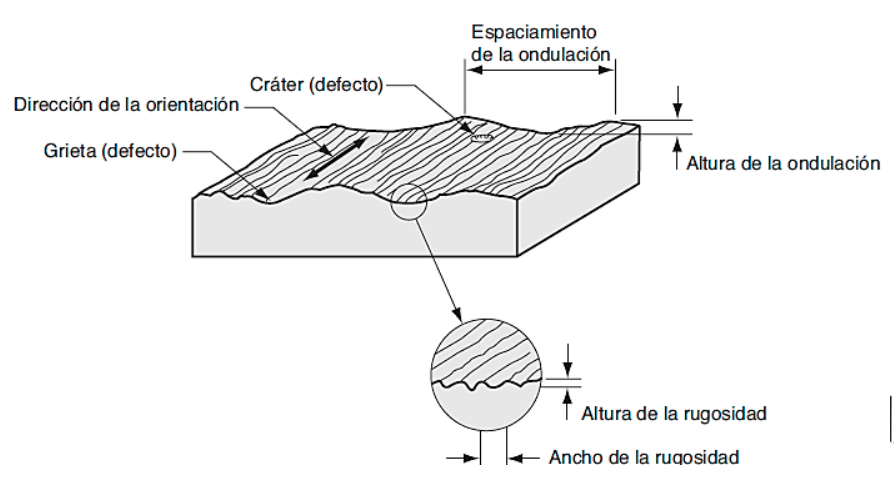
\includegraphics[width=0.8\linewidth]{img/superficie.png}
\end{figure}

\textbf{Símbolos de orientación posible:}
\begin{center}
	\small
	\begin{tabular}{@{}cp{11cm}@{}}
		\toprule
		\textbf{Símbolo} & \textbf{Significado}
		\\
		\midrule
		$=$              & Paralela a las líneas que representan la superficie a que
		se aplica
		\\
		$\perp$          & Perpendicular a la línea que representa la superficie a
		que se aplica
		\\
		X                & Angular en ambas direcciones
		\\
		M                & Multidireccional
		\\
		C                & Circular respecto al centro de la superficie
		\\
		R                & Aproximadamente radial respecto al centro de la
		superficie
		\\
		P                & Particular, no direccional o protuberante
		\\
		\bottomrule
	\end{tabular}
\end{center}

\subsubsection{Integridad de la superficie}
Es el \textbf{estudio y control de la capa subsuperficial} y cualesquiera
\textbf{cambios debidos al procesamiento} que influyan en el desempeño de la
pieza o del producto terminado.

Alteraciones superficiales y subsuperficiales que definen la integridad de una
superficie:
\begin{description}[leftmargin=0pt,style=nextline]
	\item[Absorción] Impurezas absorbidas y retenidas por las capas de la
	      superficie base del material, que pueden generar fragilidad u otros
	      cambios de
	      propiedades.
	\item[Agotamiento de la aleación] Ocurre cuando se pierden elementos críticos
	      de la aleación de la superficie o debajo de ésta, con posible pérdida de
	      propiedades.
	\item[Grietas] Rupturas o separaciones estrechas en la superficie o debajo de
	      ésta que alteran la continuidad del material; se caracterizan por
	      aristas
	      afiladas y relación de longitud a ancho de al menos 4:1. Se clasifican
	      en
	      macrogrietas (observables con ampliación de 10X o menos) y microgrietas
	      (requieren mayor ampliación).
	\item[Cráteres] Depresiones rugosas de la superficie ocasionadas por descargas
	      de cortocircuitos asociadas con métodos eléctricos de procesamiento
	      (maquinado
	      por descargas eléctricas y electroquímico).
	\item[Cambios en la dureza] Diferencias de dureza en la superficie o cerca de
	      ella.
	\item[Zona afectada por el calor (HAZ)] Región del metal afectada por la
	      aplicación de energía térmica que no funde pero se calienta lo
	      suficiente para
	      inducir cambios metalúrgicos que afectan sus propiedades. Es más
	      destacada en
	      operaciones de soldadura por fusión.
	\item[Inclusiones] Partículas pequeñas de material incorporadas a las capas de
	      la superficie durante el procesamiento; forman una discontinuidad en el
	      material
	      base.
	\item[Ataque intergranular] Varias formas de reacción química en la
	      superficie, incluyendo la corrosión y oxidación intergranular.
	\item[Traslapes, pliegues y costuras] Irregularidades y defectos en la
	      superficie ocasionados por el comportamiento plástico de superficies que
	      se
	      traslapan.
	\item[Picaduras] Depresiones poco profundas con aristas redondeadas formadas
	      por varios mecanismos, incluido grabado selectivo o corrosión; remoción
	      de
	      inclusiones superficiales; abolladuras formadas mecánicamente o acción
	      electroquímica.
	\item[Deformación plástica] Cambios microestructurales a partir de
	      deformaciones en la superficie de los metales; resultado del
	      endurecimiento por
	      deformación.
	\item[Recristalización] Formación de granos nuevos en metales endurecidos por
	      deformación; se asocia con el calentamiento de las piezas metálicas que
	      se hayan
	      deformado.
	\item[Metal redepositado] Metal removido de la superficie en estado líquido y
	      vuelto a depositar antes de solidificarse.
	\item[Metal resolidificado] Porción de la superficie que se funde durante el
	      procesamiento y después vuelve a solidificar sin abandonar la superficie
	      (también llamado metal vuelto a fundir).
	\item[Esfuerzos residuales] Esfuerzos que permanecen en el material después de
	      su procesamiento.
	\item[Grabado selectivo] Forma de ataque químico que se concentra en ciertos
	      componentes del material base.
\end{description}

% =====================================================================
\section{Semana 3: Procesos de remoción con torno}
% =====================================================================

\subsection{Definición y partes}
\begin{defi}[Torno]
	Máquina que sirve para \textbf{fabricar piezas en revolución}.
\end{defi}

\textbf{Partes del torno CNC:} \textbf{plato}, \textbf{mordazas} (sujetan la
pieza) y \textbf{torreta} (porta las herramientas), además del panel de control.

\textbf{Partes del torno paralelo:}
\begin{figure}[h!]
	\centering
	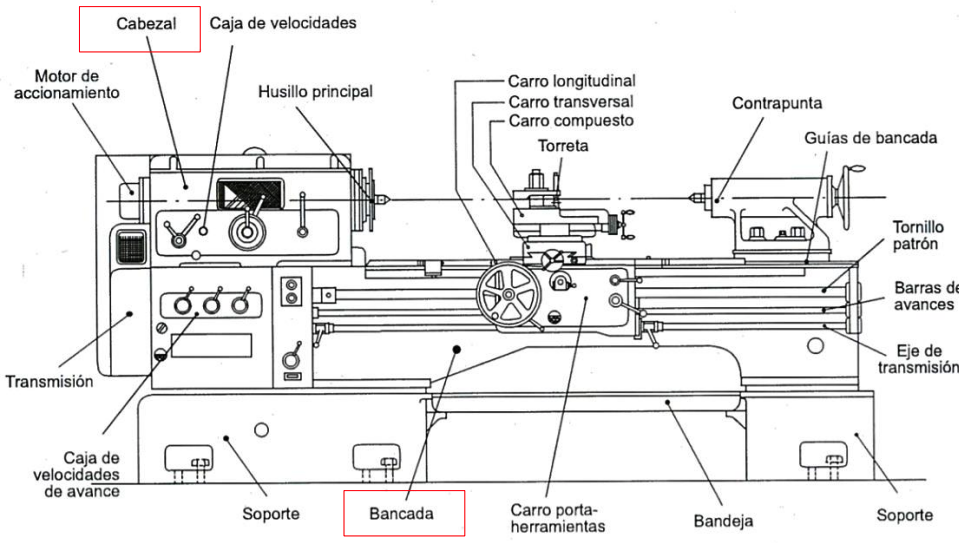
\includegraphics[width=\linewidth]{img/torno-paralelo.png}
\end{figure}

\subsection{Tipos de torno}
\begin{enumerate}
	\item \textbf{Torno paralelo:} está quedando relegado a tareas poco
	      importantes; se usa en talleres de mantenimiento para trabajos puntuales
	      o
	      especiales.
	\item \textbf{Torno copiador:} reproduce una \textbf{réplica igual a la guía}
	      (plantilla).
	\item \textbf{Torno revólver:} mecanizado para tornear piezas en las que es
	      posible el \textbf{trabajo simultáneo de varias herramientas} para
	      disminuir el
	      tiempo.
	\item \textbf{Torno automático:} realiza automáticamente las operaciones de
	      mecanizado, permitiendo una \textbf{alta productividad} y reduciendo la
	      intervención del operario.
	\item \textbf{Torno vertical:} tiene \textbf{eje vertical}; fabrica
	      \textbf{piezas de gran tamaño}.
	\item \textbf{Torno CNC:} \textbf{dirigido por computadora}; tiene gran
	      capacidad de producción y precisión en el mecanizado.
\end{enumerate}

\subsection{Procesos de torneado}
\begin{enumerate}
	\item \textbf{Cilindrado exterior:} operación para dar forma exterior y
	      \textbf{reducir el diámetro} de la barra del material.
	\item \textbf{Cilindrado interior (mandrinado):} realizar cilindros o conos
	      interiores y ranuras interiores en piezas agujereadas.
	\item \textbf{Refrentado:} mecanizar una \textbf{superficie plana
		      perpendicular al eje de giro}.
	\item \textbf{Roscado:} hacer \textbf{varias pasadas de corte} a lo largo de
	      toda la longitud de la rosca.
	\item \textbf{Ranurado:} abrir ranuras o canales en las piezas.
	\item \textbf{Tronzado:} \textbf{seccionamiento} de la barra o de una pieza
	      con una herramienta afilada llamada \emph{tronzadora}.
	\item \textbf{Moleteado:} producir una \textbf{superficie áspera o rugosa}
	      (agarre); se usan \emph{moletas} como herramienta.
	\item \textbf{Cónico:} generar superficies cónicas.
	\item \textbf{Forma:} generar perfiles según la forma de la
	      herramienta/trayectoria.
\end{enumerate}

\textbf{Herramientas} (cada proceso tiene su portaherramienta/inserto):
cilindrado, mandrilado, roscado, ranurado y tronzado.

\subsection{Desbaste vs.\ acabado}
\begin{center}
	\begin{tabularx}{\linewidth}{@{}lXX@{}}
		\toprule
		                     & \textbf{Desbaste}
		                     & \textbf{Acabado}
		\\
		\midrule
		Objetivo             & Arrancar la mayor cantidad de viruta para acercarse a
		la medida final
		                     & Trabajo casi superficial; da las tolerancias
		adecuadas; se torna hasta la
		medida final
		\\
		Velocidad de corte   & \textbf{baja}
		                     & \textbf{alta}
		\\
		Avance               & \textbf{alto}
		                     & \textbf{bajo}
		\\
		Profundidad de corte & \textbf{grande}
		                     & \textbf{pequeña}
		\\
		Tiempo de mecanizado & \textbf{bajo}
		                     & \textbf{alto}
		\\
		\bottomrule
	\end{tabularx}
\end{center}
Por tanto: $v_D < v_A$, $a_D > a_A$ y $n_D < n_A$ (subíndice D = desbaste, A =
acabado).

\subsection{Parámetros del torneado}

\begin{formu}[1. Velocidad de corte]
	\[ v = n\left(\frac{D_i}{2}\right) \]
	$v$ = velocidad de corte (m/min); $n$ = velocidad de giro o angular del chuck
	(rev/min = rpm), con 1 rev $= 2\pi$; $D_i$ = diámetro inicial (mm).\\
	En la práctica: $v = \dfrac{\pi\, D_i\, n}{1000}$ con $D_i$ en mm y $v$ en
	m/min
	(el factor $2\pi$ convierte revoluciones a radianes y el 1000 pasa mm a m).
\end{formu}

\begin{formu}[2. Velocidad lineal (de avance)]
	\[ v_L = n\cdot a \]
	$v_L$ = velocidad lineal o de avance; $n$ = rpm; $a$ = avance (mm/rev). Con
	$a$
	en mm/rev el resultado queda en mm/min.
\end{formu}

\begin{formu}[3. Caudal de viruta]
	\[ Q = v_L \cdot A \qquad (Q = V/t) \]
	$V$ = volumen, $t$ = tiempo, $v_L$ = velocidad lineal o de avance, $A$ = área
	de la sección de material removido (área de la corona circular en cilindrado:
	$A
		= \tfrac{\pi}{4}(D_i^2 - D_f^2)$).
\end{formu}

\begin{formu}[4. Profundidad de corte o de pasada]
	\[ p_T = \frac{D_i - D_f}{2} \qquad\qquad p_T = N_D P_D + N_A P_A \]
	$p_T$ = profundidad total; $N_A$, $N_D$ = número de pasadas de acabado y de
	desbaste; $P_D$, $P_A$ = profundidad de desbaste y de acabado. \textbf{El
		número
		de pasadas debe ser entero.}\\
	Rangos: \textbf{acabado} $P_A \approx 0.1$--$0.5$ mm;
	\textbf{desbaste} $P_D \approx 0.4$--$3$ mm.\\
\end{formu}

\begin{formu}[5. Tiempo de pasada]
	\[ t_p = \frac{L + y + \Delta}{v_L} = \frac{L + y + \Delta}{a\cdot n} \]
	$L$ = longitud a mecanizar; $y$ = retiro de cuchilla (1--3 mm); $\Delta$ =
	distancia por efecto del ángulo de posición $\omega$, con $\tan\omega =
		p/\Delta$.\\
	Si $\omega = 45^\circ \Rightarrow \Delta = p$; si $\omega = 90^\circ
		\Rightarrow \Delta = 0$.
\end{formu}

\begin{formu}[6. Tiempo de maquinado]
	\[ t_m = N\left(\frac{L + y + \Delta}{a\cdot n}\right) \]
	$N$ = número de pasadas. Si hay desbaste y acabado con parámetros distintos,
	se suman los tiempos de cada etapa: $t_m = t_D + t_A$.
\end{formu}

\begin{table}[H]
	\centering
	\small
	\caption{Tabla de velocidades de corte $v$ (m/min)}
	\vspace{10pt}
	\begin{tabular}{@{}lcccc@{}}
		\toprule
		                          & \multicolumn{2}{c}{\textbf{Acero rápido}} &
		\multicolumn{2}{c}{\textbf{Pastilla carburada}}
		\\
		\textbf{Material del eje} & Desbaste                                  &
		Acabado                   & Desbaste                                  &
		Acabado
		\\
		\midrule
		Acero 0.35 \%C            & 25                                        & 30
		                          & 200                                       & 300
		\\
		Acero 0.45 \%C            & 15                                        & 20
		                          & 120                                       & 160
		\\
		Acero extra duro          & 12                                        & 16
		                          & 40                                        & 60
		\\
		Hierro fundido maleable   & 20                                        & 25
		                          & 70                                        & 85
		\\
		Hierro fundido gris       & 15                                        & 20
		                          & 65                                        & 95
		\\
		Hierro fundido duro       & 10                                        & 15
		                          & 30                                        & 50
		\\
		Bronce                    & 30                                        & 40
		                          & 300                                       & 380
		\\
		Latón y cobre             & 40                                        & 50
		                          & 350                                       & 400
		\\
		Aluminio                  & 60                                        & 90
		                          & 500                                       & 700
		\\
		Fibra y ebonita           & 25                                        & 40
		                          & 120                                       & 150 \\
		\bottomrule
	\end{tabular}
\end{table}
Observa que: la pastilla carburada permite velocidades mucho mayores que el
acero rápido; el acabado siempre usa más velocidad que el desbaste; y los
materiales blandos (aluminio, latón, cobre, bronce) se cortan a mayor velocidad
que los aceros y fundiciones duras.

\subsection{Ejercicios resueltos}

\subsubsection*{Ejercicio 1: cilindrado de una pieza}
\textbf{Enunciado:} cilindrar una pieza de $D = 100$ mm a $d = 88$ mm, $L = 200$
mm. Torno con $n_D = 130$ rpm (desbaste) y $n_A = 235$ rpm (acabado), avance $a
	= 0.3$ mm/rev. Profundidad de desbaste 4 mm y de acabado 2 mm; útil
perpendicular a la pieza ($\omega = 90^\circ$, $\Delta = 0$); retiro $y = 3$ mm.

\textbf{a) Velocidad de corte de desbaste:}
\[ v_D = n_D\frac{D_{iD}}{2} = 130\,\frac{\text{rev}}{\text{min}}\cdot\frac{100\
		\text{mm}}{2}\cdot\frac{2\pi}{1\ \text{rev}}\cdot\frac{1\ \text{m}}{1000\
		\text{mm}} = \mathbf{40.84\ m/min} \]

\textbf{b) Velocidad de corte de acabado:} diámetro inicial del acabado $D_{iA}
	= D_f + 2P_A = 88 + 2(2) = 92$ mm.
\[ v_A = 235\cdot\frac{92}{2}\cdot 2\pi\cdot\frac{1}{1000} = \mathbf{67.92\
		m/min} \]

\textbf{c) Número de pasadas de desbaste:}
\[ \frac{100-88}{2} = 6 = N_A P_A + N_D P_D = 1(2) + N_D P_D \]
La solución manuscrita de la diapositiva usa $P_D = 3$ mm: $N_D = 4/3 = 1.33
	\approx 2$ pasadas.

\textbf{d) Velocidad de giro recomendada} si $v = 40$ m/min:
\[ n = \frac{2v}{D_i} = \frac{40\ \text{m/min}\cdot 1000}{\pi\cdot 100\
		\text{mm}} = 127.3\ \text{rpm} \;\Rightarrow\; \text{de la tabla se
		recomienda }
	\mathbf{130\ rpm} \]
(se elige la velocidad disponible más cercana).

\textbf{e) Tiempo de maquinado del desbaste:}
\[ t_D = N_D\left[\frac{L + y + \Delta}{a\, n_D}\right] = 1\left[\frac{200 + 3 +
			0}{0.3\cdot 130}\right] = \mathbf{5.2\ min} \]

\begin{aviso}[Inconsistencia en la solución de las diapositivas]
	El enunciado dice \textbf{$P_D = 4$ mm}, pero la solución manuscrita usa $P_D
		= 3$ mm en (c) y obtiene 1.33 $\approx$ 2 pasadas, mientras que en (e) usa
	\textbf{$N_D = 1$}. Con $P_D = 4$ mm del enunciado: $6 = 2 + N_D(4)
		\Rightarrow
		N_D = 1$ pasada exacta, que sí es coherente con (e). Para el examen,
	asegúrate
	de usar los datos del enunciado que te den y de verificar que el número de
	pasadas resulte entero.
\end{aviso}

\subsubsection*{Ejercicio 2: barra de 60 mm a 48.4 mm}
\textbf{Enunciado:} barras de 237 mm de largo y 60 mm de diámetro, a cilindrar
hasta 48.4 mm. Avances 0.2 y 0.8 mm/rev; velocidades de rotación 128 y 207 rpm.
Se programan \textbf{3 pasadas de desbaste} de igual profundidad a lo largo de
207 mm (se deja un exceso de 30 mm para la sujeción al chuck) y \textbf{1 pasada
	de acabado} de 0.4 mm. Determinar: (a) $v_D$, (b) $v_A$, (c) caudal de viruta
de
la primera pasada de desbaste en cm$^3$/min.

\textbf{Asignación de datos} (recuerda: $v_D<v_A$, $a_D>a_A$, $n_D<n_A$): $a_D =
	0.8$, $a_A = 0.2$ mm/rev; $n_D = 128$, $n_A = 207$ rpm; $N_D = 3$, $N_A = 1$,
$P_A = 0.4$ mm.

\textbf{a)} $v_D = 128\cdot\dfrac{60}{2}\cdot 2\pi\cdot\dfrac{1}{1000} =
	\mathbf{24.13\ m/min}$.

\textbf{b)} Profundidad total: $P = \dfrac{60 - 48.4}{2} = 5.8$ mm. De $5.8 =
	3P_D + 1(0.4)$ resulta $P_D = 1.8$ mm. Cada pasada de desbaste reduce el
diámetro en $2(1.8) = 3.6$ mm: $D_{i2D} = 56.4$, $D_{i3D} = 52.8$, y el diámetro
inicial del acabado es $D_{iA} = 60 - 6(1.8) = 49.2$ mm.
\[ v_A = 207\cdot\frac{49.2}{2}\cdot 2\pi\cdot\frac{1}{1000} = \mathbf{32\
		m/min} \]

\textbf{c)} Caudal en la primera pasada de desbaste:
\[ Q = v_L\cdot A = (a_D n_D)\cdot\frac{\pi}{4}(60^2 - 56.4^2) = (0.8\cdot
	128)(329.1\ \text{mm}^2) \approx 33\,700\ \text{mm}^3/\text{min} =
	\mathbf{33.7\
		cm^3/min} \]

\subsubsection*{Ejercicio 3: cilindrado interior y tronzado de un bloque hueco
	SAE 1045}
\textbf{Enunciado:} bloque cilíndrico hueco SAE 1045, $D_{ext} = 100$ mm,
$D_{int} = 64$ mm, longitud 250 mm. Cilindrado interior con profundidad total de
2 mm: 3 pasadas de desbaste de 0.6 mm y 1 de acabado. Pastilla carburada.
Velocidades angulares 217.03 rpm (desbaste) y 323.34 rpm (acabado); avances
0.2032 mm/rev (desbaste) y 0.016 mm/rev (acabado). Luego se tronza la pieza.

\textbf{a) Diámetro inicial y profundidad del acabado.} $2 = 3(0.6) + 1\cdot P_A
	\Rightarrow P_A = \mathbf{0.2\ mm}$. En un cilindrado \emph{interior} el
diámetro crece: $D_{1D} = 64$, $D_{2D} = 65.2$, $D_{3D} = 66.4$, $D_{iA} = 64 +
	6(0.6) = \mathbf{67.6\ mm}$, y el diámetro final es $D_f = 68$ mm.

\textbf{b) Caudal de viruta de la pasada de acabado:}
\[ Q_A = a_A\, n_A\cdot\frac{\pi}{4}(68^2 - 67.6^2) = 0.016\cdot
	323.34\cdot\frac{\pi}{4}(54.24) \approx \mathbf{220.4\ mm^3/min} = 0.22\
	\text{cm}^3/\text{min} \]

\textbf{c) Tiempo de pasada para tronzar} (rpm y avance del desbaste). Tras el
cilindrado el bloque queda con $D_{ext} = 100$ y $D_{int} = 68$; en el tronzado
de un cilindro hueco, $L = \dfrac{D_f - D_i}{2} = \dfrac{100-68}{2} = 16$ mm,
con $\omega = 90^\circ$ ($\Delta = 0$) y $y = 2$ mm:
\[ t_p = \frac{16 + 2 + 0}{0.2032\cdot 217.03} = \mathbf{0.408\ min} \]

\subsubsection*{Ejercicio 4: refrentado de una pieza maciza SAE 1035 de 300 mm}
\textbf{Enunciado:} refrentado con $n = 48$ rpm hasta alcanzar $D = 200$ mm;
luego 74 rpm hasta $D = 100$ mm; luego 116 rpm hasta el centro. Avance $a = 0.2$
mm/rev, retiro $y = 2$ mm, $\Delta = 0$ (herramienta a ángulo recto). Calcular:
(a) tiempo de maquinado total, (b) tiempo de maquinado y tiempo ahorrado si no
se cambia la velocidad angular, (c) caudal de viruta del primer tramo en
cm$^3$/min (despreciando la profundidad de refrentado).

En refrentado la longitud recorrida por la herramienta es el radio a eliminar en
cada tramo:

\textbf{a)}
\begin{align*}
	t_1     & = \frac{\frac{300-200}{2} + 2 + 0}{0.2\cdot 48} = \frac{52}{9.6} =
	5.42\
	\text{min}
	\\
	t_2     & = \frac{\frac{200-100}{2} + 2 + 0}{0.2\cdot 74} = \frac{52}{14.8} =
	3.51\
	\text{min}
	\\
	t_3     & = \frac{\frac{100-0}{2} + 2 + 0}{0.2\cdot 116} = \frac{52}{23.2} =
	2.24\ \text{min}
	\\
	t_{maq} & = t_1 + t_2 + t_3 = \mathbf{11.17\ min}
\end{align*}

\textbf{b)} Sin cambiar la velocidad (48 rpm todo el recorrido): $t = \dfrac{150
		+ 2 + 0}{0.2\cdot 48} = 15.83$ min. Tiempo ahorrado $= 15.83 - 11.17 =
	\mathbf{4.66\ min}$.

\textbf{c)} $v_L = a\,n = 0.2\cdot 48 = 9.6$ mm/min; $A = \dfrac{\pi}{4}(300^2 -
	200^2) = 39\,269.9$ mm$^2$.
\[ Q = v_L A = 9.6\cdot 39\,269.9 \approx 376\,990\ \text{mm}^3/\text{min}
	\approx \mathbf{377\ cm^3/min} \]

\begin{aviso}[Error numérico en las diapositivas]
	Las diapositivas escriben $t_{maquinado} = 10.81$ min y ahorro $= 5.02$ min.
	Sin embargo, $5.42 + 3.51 + 2.24 = 11.17$ min (no 10.81) y por tanto el ahorro
	es $15.83 - 11.17 = 4.66$ min. El \textbf{método} es el correcto; solo la suma
	final está mal en el material. Si tu examen incluye este ejercicio, usa los
	valores recalculados aquí.
\end{aviso}

% =====================================================================
\newpage
\section{Semana 4: Fresado}
% =====================================================================

\textbf{Contenidos:} introducción (características del proceso y tipos de
piezas, descripción del proceso), operaciones y herramientas comunes,
herramientas de fresado (partes, ángulos de los filos, acción de cada diente),
parámetros de fresado (básicos, avance por diente y espesor de viruta, sección
de viruta, fuerza de corte, potencia de corte), fresadoras (descripción y
arquitecturas) y cuestionario.

\subsection{Introducción}

\subsubsection{Características del proceso y tipos de piezas}
Operaciones de mecanizado para piezas de geometría diversa: piezas prismáticas,
complejas, superficies inclinadas, superficies planas y acabado de zonas de
piezas fundidas/forjadas; también piezas de geometría compleja como
\textbf{moldes, matrices, álabes y piezas aeronáuticas}.

\begin{center}
	\begin{tabular}{@{}p{7.3cm}p{7.3cm}@{}}
		\toprule
		\textbf{Ventajas}
		                                                                            &
		\textbf{Limitaciones}
		\\
		\midrule
		\begin{itemize}[leftmargin=10pt,nosep]
			\item Cualquier geometría.
			\item Buena precisión y acabado superficial comparado con fundición/forja.
			\item Flexibilidad: desde piezas unitarias hasta largas series.
			\item Diferentes materiales (con limitación en materiales muy duros).
		\end{itemize} &
		\begin{itemize}[leftmargin=10pt,nosep]
			\item Proceso caro.
			\item Limitado en algunos materiales muy difíciles de trabajar.
		\end{itemize}               \\
		\bottomrule
	\end{tabular}
\end{center}

\subsubsection{Descripción del proceso}
\begin{itemize}
	\item \textbf{Aplicación:} mecanizado de piezas \textbf{sin simetría de
		      revolución} (en contraste con el torno).
	\item Se combinan \textbf{dos movimientos}: el \textbf{movimiento principal o
		      de corte} y el \textbf{movimiento de avance}.
	\item \textbf{Movimiento principal:} \textbf{giro de la herramienta}. Consume
	      la mayor potencia y tiene velocidad mayor que el de avance.
	\item \textbf{Movimiento de avance:} lo más común es una fresadora de
	      \textbf{3 grados de libertad (XYZ)}. Por cada giro de la fresa, ésta
	      solo avanza
	      del orden de 0.1--0.2 mm.
	\item \textbf{Proceso muy versátil por dos motivos:} posibilidad de
	      \textbf{variar la dirección} del movimiento de avance y posibilidad de
	      \textbf{cambiar la geometría de la fresa}.
\end{itemize}

\subsection{Operaciones comunes}
\begin{itemize}
	\item \textbf{Planeado:} obtener superficies planas.
	\item \textbf{Escuadrado:} obtener superficies perpendiculares entre sí
	      (escuadras/escalones).
	\item \textbf{Mecanizado de cajeras:} vaciados interiores; requiere
	      \textbf{fresas con filo al centro}.
	\item \textbf{Mecanizado de superficies complejas:} contornos 3D, moldes,
	      matrices.
\end{itemize}

\subsection{Herramientas de fresado}
\textbf{Partes de una herramienta:} se divide en \textbf{mango} y \textbf{parte
	cortante}. En la parte cortante suele haber varios filos, y en cada uno se
distinguen:
\begin{itemize}
	\item \textbf{Filo principal} y \textbf{filo secundario}.
	\item \textbf{Superficie de incidencia} y \textbf{superficie de
		      desprendimiento}.
	\item \textbf{Punta del diente}.
	\item \textbf{Alojamiento para la viruta}.
	\item En fresas con insertos: \textbf{plaquita de asiento} y \textbf{plaquita
		      de corte}.
\end{itemize}

\textbf{Ángulos de los filos de una fresa:}
\begin{itemize}
	\item Ángulo de posición del filo principal ($\kappa_r$).
	\item Ángulo de posición del filo secundario ($\kappa'_r$).
	\item Ángulo de desprendimiento ($\gamma$), que se descompone en
	      \textbf{axial} ($\gamma_a$) y \textbf{radial} ($\gamma_r$).
	\item Ángulo de incidencia ($\alpha$).
\end{itemize}
Según los signos de $\gamma_a$ y $\gamma_r$ hay tres tipos de geometría:
\textbf{doblemente negativa}, \textbf{positiva--negativa} y \textbf{doblemente
	positiva}. \textbf{Hacia la doblemente negativa} $\Rightarrow$ \textbf{mayor
	robustez del filo}; \textbf{hacia la doblemente positiva} $\Rightarrow$
\textbf{mejor flujo de la viruta}.

\textbf{Acción de cada diente en la pieza:} los filos giran y se trasladan
simultáneamente, por lo que se genera un \textbf{corte intermitente}: el filo
entra y sale de la pieza, y la \textbf{cantidad de material que arranca varía
	según la posición angular}.

\subsection{Parámetros de fresado}

\begin{formu}[Parámetros básicos]
	\textbf{Velocidad de corte (m/min):}
	\[ V_c = \frac{\pi\, D\, N}{1000} \]
	$D$ = diámetro de la fresa (mm); $N$ = velocidad de rotación (rpm).
	(Despejando:
	$N = \dfrac{1000\,V_c}{\pi D}$.)\\[4pt]
	\textbf{Profundidades de pasada:} radial $a_e$ y axial $a_p$ (mm).\\[4pt]
	\textbf{Velocidad de avance:} $V_f$ (mm/min).\\[4pt]
	\textbf{Avance por filo (mm/filo):}
	\[ f_z = \frac{V_f}{N\, z} \qquad\left(V_f = f_z\, N\, z\right) \]
	$z$ = número de filos de la fresa.
\end{formu}

\begin{formu}[Espesor de viruta]
	El espesor de viruta $a_c$ \textbf{varía a lo largo del recorrido del diente};
	depende de la posición angular $\psi$ del diente.\\[3pt]
	Si $\kappa_r = 90^\circ$: $\quad a_c = f_z \sin\psi \quad$ y el máximo es
	$a_{c,max} = f_z$.\\[3pt]
	Si $\kappa_r \neq 90^\circ$: $\quad a_c = f_z \sin\psi\,\sin\kappa_r$.
\end{formu}

\begin{formu}[Sección de viruta]
	Sección de material arrancada por un diente = espesor de corte $\times$
	anchura de corte:
	\[ S_c = a_c \cdot a_w \]
	Como el espesor varía en cada instante, \textbf{la sección de viruta también
		varía}.
\end{formu}

\begin{formu}[Fuerza de corte]
	\[ F_c = p_s \cdot S_c \]
	$p_s$ = presión (energía) específica de corte. Al igual que en torneado
	depende del material y de los parámetros de corte. \textbf{En fresado es
		variable por dos motivos:} $S_c$ es variable y $p_s$ es función de $a_c$,
	que
	también varía. Se descompone en fuerza \textbf{axial} $F_a$, \textbf{radial}
	$F_r$ y de corte $F_c$. La fuerza varía periódicamente en el tiempo (golpes de
	cada diente) y puede cambiar de signo.\\
	La curva $p_s(a_c)$ muestra la zona habitual de fresado (espesores de viruta
	pequeños) frente a la de torneado (espesores mayores).
\end{formu}

\begin{formu}[Potencia de corte]
	Como $F_c$ es variable con el tiempo y puede haber varios dientes en corte a
	la vez, no es posible un cálculo simple:
	\[ P_c = F_c(t)\, V_c = S_c(t)\, p_s(a_c)\, V_c = a_c(t)\, a_w\, p_s(a_c(t))\,
		V_c \quad \text{(¡cálculo complicado!)} \]
	Por eso se calcula un \textbf{valor medio} con el valor medio de la energía
	específica de corte $p_s^*$ (se obtiene de tablas a partir del espesor medio
	de
	corte $\bar a_c$) multiplicado por el volumen de viruta mecanizado por unidad
	de
	tiempo:
	\[ P_m = p_s^*(\bar a_c)\, V_f\, a_p\, a_e \qquad\quad \bar a_c =
		\frac{1}{\Theta}\int_0^{\Theta} a_c\, d\theta = \frac{2\, a_e\, f_z\,
			\sin\kappa_r}{\Theta\, D} \]
	Nótese que $V_f\, a_p\, a_e$ es el \textbf{caudal de viruta} $Q$ (volumen
	removido por unidad de tiempo), de modo que $P = p_s\cdot Q$.
\end{formu}

\subsection{Fresadoras}
La \textbf{fresadora} es la máquina-herramienta que lleva a cabo el proceso de
fresado.

\textbf{Partes:} \textbf{cabezal}, \textbf{herramienta}, \textbf{mesa},
\textbf{columna}, \textbf{carro}, \textbf{guías} y \textbf{consola}.

\textbf{La fresadora debe aportar:}
\begin{itemize}
	\item Giro de la fresa a diferentes velocidades y con potencia suficiente.
	\item Movimiento de avance relativo entre herramienta y pieza en cualquier
	      dirección.
	\item Además: movimientos \textbf{precisos} y sujeción de la pieza y de las
	      herramientas con fuerza suficiente.
\end{itemize}

\textbf{Tipos:} a diferencia de otras máquinas-herramienta, existen
\textbf{muchos tipos de fresadoras} según el tipo y tamaño de pieza a mecanizar.
\begin{itemize}
	\item \textbf{Manuales:} los movimientos de avance se logran con sistemas
	      mecánicos accionados a mano.
	\item \textbf{CN (control numérico):} los avances son accionados por
	      \textbf{servomotores} que ejecutan un programa.
	\item Según la orientación del eje de la fresa: \textbf{eje vertical} o
	      \textbf{eje horizontal}.
	\item Existen \textbf{7 arquitecturas} de fresadoras de 3 ejes (según qué
	      elemento mueve cada eje: mesa, columna, cabezal, etc.).
\end{itemize}

\subsection{Cuestionario tutorizado (con ideas de respuesta)}
Las diapositivas solo plantean las preguntas; las respuestas siguientes son
\emph{orientativas} para que practiques.
\begin{enumerate}
	\item \textbf{Geometrías difíciles o imposibles de fresar:} cavidades internas
	      cerradas sin acceso para la herramienta, huecos profundos y estrechos
	      (la
	      herramienta no cabe o se flexiona), esquinas internas con radio menor al
	      de la
	      fresa, y socavados sin acceso.
	\item \textbf{Número máximo de ejes:} suelen incorporar hasta \textbf{5 ejes}.
	      Ventajas: mecanizar geometrías complejas en una sola sujeción, mejor
	      acabado y
	      accesibilidad. Desventajas: mayor costo, programación más compleja y
	      riesgo de
	      colisiones.
	\item \textbf{Viruta en fresado:} el corte es \textbf{intermitente}; cada
	      diente produce una viruta corta y discontinua, que se desprende
	      fácilmente, a
	      diferencia del torneado donde la viruta es continua y puede enredarse.
	\item \textbf{Rugosidad:} la secuencia de golpes de los filos deja una marca
	      por cada avance por filo; la rugosidad aumenta con el avance por filo
	      $f_z$ (y
	      disminuye con el radio de punta). El parámetro más influyente es el
	      \textbf{avance por filo} $f_z$.
	\item \textbf{Componentes de la fuerza:} la \textbf{tangencial} (la de corte)
	      genera el par y determina la potencia; la \textbf{radial}
	      empuja/flexiona la
	      herramienta o la pieza y afecta a la precisión dimensional y a las
	      vibraciones.
	\item \textbf{Fresadora horizontal vs.\ vertical:} mejor evacuación de la
	      viruta por gravedad y posibilidad de emplear fresas tipo disco o varias
	      fresas
	      en el mismo árbol.
	\item \textbf{Mesa inmóvil y herramienta móvil:} no hay que mover el peso de
	      la pieza (útil en piezas grandes y pesadas), lo que mejora la dinámica y
	      la
	      precisión.
\end{enumerate}

\subsection{Ejercicios resueltos}

\subsubsection*{Ejercicio 1: velocidad de rotación}
Fresa de carburo de $D = 80$ mm para acero, $V_c = 120$ m/min.
\[ N = \frac{V_c\cdot 1000}{\pi\, D} = \frac{120\cdot 1000}{\pi\cdot 80} =
	\frac{120\,000}{251.33} \approx \mathbf{477.46\ rpm} \]

\subsubsection*{Ejercicio 2: tiempo de una pasada de fresado frontal}
Placa de aluminio, $L = 300$ mm; longitud de aproximación y salida total $A =
	25$ mm; velocidad de avance $f = V_f = 250$ mm/min.
\[ T_m = \frac{L + A}{V_f} = \frac{300 + 25}{250} = \frac{325}{250} =
	\mathbf{1.3\ min}\ (78\ \text{s}) \]

\subsubsection*{Ejercicio 3: potencia de corte}
Tasa de remoción $Q = 45\ \text{cm}^3/\text{min} = 0.45\times 10^{-4}\
	\text{m}^3/\text{min}$; presión específica de corte $K_s = 2000\
	\text{N/mm}^2$.
\[ P_c = K_s\, Q = 2000\ \tfrac{\text{N}}{\text{mm}^2}\cdot 750\
	\tfrac{\text{mm}^3}{\text{s}} = 1.5\times 10^{6}\
	\tfrac{\text{N}\cdot\text{mm}}{\text{s}} = 1500\ \text{W} = \mathbf{1.5\ kW} \]
(Conversión: $45\ \text{cm}^3/\text{min} = 45\,000\ \text{mm}^3/60\ \text{s} =
	750\ \text{mm}^3/\text{s}$. En el sistema SI: $2000\times10^6\ \text{N/m}^2
	\cdot 0.45\times10^{-4}\ \text{m}^3/\text{min} = 9\times10^4\ \text{N·m/min} =
	1500\ \text{W}$.)

\begin{aviso}[Sobre la solución de este ejercicio en las diapositivas]
	La imagen de la solución del ejercicio 3 tiene texto desordenado (aparece una
	``wait, conversión fact\ldots'' a medio escribir). El resultado correcto es
	\textbf{1.5 kW}, como se muestra arriba; ignora el resto del texto confuso.
\end{aviso}

Las diapositivas que siguen a estos ejercicios están vacías (solo el título
``EJERCICIOS''). Cierran con empresas y productos que usan fresado: matrices de
estampación, piezas aeronáuticas de fuselaje, piezas de precisión, rodetes de
turbinas para el sector hidroeléctrico y satélites.

% =====================================================================
\newpage
\section{Hoja resumen de fórmulas y conceptos clave}
% =====================================================================

\subsection{Fórmulas de tolerancias y ajustes}
\begin{center}
	\small
	\begin{tabular}{@{}ll@{}}
		\toprule
		\textbf{Concepto}       & \textbf{Fórmula}
		\\
		\midrule
		Tolerancia del agujero  & $T = D_M - D_m = D_s - D_i$
		\\
		Tolerancia del eje      & $t = d_M - d_m = d_s - d_i$
		\\
		Dimensiones límite      & $D_M = D_N + D_s$, $D_m = D_N + D_i$ (igual para
		ejes con minúsculas)
		\\
		Juego                   & $J = D_e - d_e > 0$; $J_M = D_M - d_m$; $J_m = D_m
			                                                                  - d_M$;
		$T_J = T + t$
		\\
		Aprieto                 & $A = d_e - D_e > 0$; $A_M = d_M - D_m$; $A_m = d_m
			                                                                  - D_M$;
		$T_A = T + t$
		\\
		Indeterminado           & $J_M = D_M - d_m$; $A_M = d_M - D_m$; $T_I = J_M +
			                                                                A_M = T +
			                                                                t$ \\
		Agujero base / eje base & Agujero H ($D_i = 0$) / eje h ($d_s = 0$)
		\\
		\bottomrule
	\end{tabular}
\end{center}

\subsection{Fórmulas de torneado}
\begin{center}
	\small
	\begin{tabular}{@{}ll@{}}
		\toprule
		\textbf{Concepto}   & \textbf{Fórmula}
		\\
		\midrule
		Velocidad de corte  & $v = n\,\dfrac{D_i}{2}$ (en práctica $v = \pi D_i
			                                                           n/1000$ en
		m/min con $D_i$ en mm)
		\\[6pt]
		Velocidad lineal    & $v_L = n\, a$
		\\[3pt]
		Caudal de viruta    & $Q = v_L\, A$
		\\[3pt]
		Profundidad total   & $p_T = \dfrac{D_i - D_f}{2} = N_D P_D + N_A P_A$
		\\[6pt]
		Tiempo de pasada    & $t_p = \dfrac{L + y + \Delta}{a\, n}$
		\\[6pt]
		Tiempo de maquinado & $t_m = N\,\dfrac{L + y + \Delta}{a\, n}$
		\\
		Ángulo de posición  & $\omega = 90^\circ \Rightarrow \Delta = 0$; $\omega =
			                                                                  45^\circ
			                                                                  \Rightarrow
			                                                                  \Delta =
			                                                                  p$
		\\
		Cilindrado interior & El diámetro inicial va \emph{creciendo}: $D_i =
			                                                               D_{int} +
			                                                               2(\text{profundidad
				                                                               acumulada})$
		\\
		\bottomrule
	\end{tabular}
\end{center}

\subsection{Fórmulas de fresado}
\begin{center}
	\small
	\begin{tabular}{@{}ll@{}}
		\toprule
		\textbf{Concepto}  & \textbf{Fórmula}
		\\
		\midrule
		Velocidad de corte & $V_c = \dfrac{\pi D N}{1000}$ (m/min)
		\\[6pt]
		Avance por filo    & $f_z = \dfrac{V_f}{N z}$
		\\[6pt]
		Espesor de viruta  & $a_c = f_z\sin\psi$ ($\kappa_r = 90^\circ$); $a_c =
			                                                                  f_z\sin\psi\sin\kappa_r$
		($\kappa_r \ne 90^\circ$)
		\\[3pt]
		Sección de viruta  & $S_c = a_c\, a_w$
		\\[3pt]
		Fuerza de corte    & $F_c = p_s\, S_c$
		\\[3pt]
		Potencia media     & $P_m = p_s^*(\bar a_c)\, V_f\, a_p\, a_e$ ($=p_s\cdot
			                                                                Q$)
		\\[3pt]
		Tiempo de pasada   & $T_m = \dfrac{L + A}{V_f}$
		\\
		\bottomrule
	\end{tabular}
\end{center}

\subsection{Ideas que suelen preguntarse}
\begin{itemize}
	\item \textbf{Cristalino vs.\ amorfo:} orden de largo alcance vs.\ desorden.
	      Las tres redes metálicas más comunes: BCC, FCC y HCP.
	\item \textbf{Clasificación de defectos por dimensión:} puntuales (vacante,
	      intersticial, sustitucional, Frenkel, Schottky), lineales (arista,
	      hélice,
	      mixta), planares (bordes de grano, maclas, límites de fase) y
	      volumétricos
	      (poros, grietas, inclusiones).
	\item \textbf{Frenkel vs.\ Schottky:} vacante + intersticial (el ion sigue en
	      el cristal) vs.\ par de vacantes catión--anión (neutralidad).
	\item \textbf{Las dislocaciones} explican la deformación plástica (ductilidad
	      y maleabilidad) de los metales.
	\item \textbf{Tolerancia} = diferencia entre límites máximo y mínimo.
	      Bilateral, unilateral y límite.
	\item \textbf{Posición de la tolerancia:} H ($D_i = 0$) y h ($d_s = 0$). A
	      menor IT, mayor precisión.
	\item \textbf{Ajustes:} con juego ($J>0$), con aprieto ($A>0$) o
	      indeterminado; en los tres $T_{ajuste} = T + t$.
	\item \textbf{Superficie:} textura (rugosidad, ondulación, orientación,
	      defectos) e integridad (alteraciones de la capa subsuperficial).
	\item \textbf{Desbaste vs.\ acabado:} desbaste $\to$ $v$ baja, avance alto,
	      profundidad grande; acabado $\to$ $v$ alta, avance bajo, profundidad
	      pequeña.
	\item \textbf{Torno vs.\ fresadora:} el torno hace piezas de revolución (gira
	      la pieza); la fresadora mecaniza piezas sin simetría de revolución (gira
	      la
	      herramienta, corte intermitente).
\end{itemize}

\end{document}
